\chapter{Evaluation\label{cha:chapter6}}
This chapter structures in two parts. First, risks and tradeoffs of the concept and implementation are illuminated with an established SOA evaluation method. Second, RG is discussed and possible improvements are pointed out.

\section{The ATAM Method}
\epigraph{It is better to be vaguely right than exactly wrong.}{Carveth Read (1848 – 1931) philosopher and logician}
In this chapter, an excerpt of the architecture tradeoff analysis method (ATAM,~\cite{Kazman1998TheMethod}) as conducted in~\cite{Bianco2007EvaluatingArchitecture} shall be used to evaluate the current implementation and underlying concept. ATAM is a method aimed at illuminating risks in the architecture through the identification of attribute trends, rather than at precise characterizations of measurable quality attribute values~\cite{Kazman1999ExperienceAnalysis}. ATAM focuses on the analysis of quality attributes. Quality attributes, also known as \textbf{nonfunctional requirements}, include usability, performance, scalability, reliability, security and modifiability. Subsection~\ref{subseb:qualatt} provides some generic examples. Subsections~\ref{subsec:atamsteps} and~\ref{subsec:atamgoa} introduce the necessary ATAM steps and the goal of finding risks and tradeoffs. For the introduced framework it is an applicable method as it stays high level. Once it is implemented in an industrial environment, a more quantifiable method is necessary.  

ATAM has been introduced by Kazman in 1998 at Carnegie Mellon University in Pennsylvania~\cite{Kazman1998TheMethod}. It was used on at least 18 architectures in the 2000s~\cite{Bass2007RiskEvaluations}. In 2013, Zalewski introduced an updated ATAM method which can be applied at an even earlier stage of architecture evaluation~\cite{Zalewski2013BeyondSystems}.

\subsection{Quality Attributes}
\label{subseb:qualatt}
The following example quality attributes are decorated with generic examples which are directly quoted from Appendix A in \textit{Evaluating a Service-Oriented Architecture}~\cite{Bianco2007EvaluatingArchitecture}.
\subsubsection{Performance}
\begin{itemize}
    \item A sporadic request for service ‘X’ is received by the server during normal operation. The system processes the request in less than ‘Y’ seconds. 
    \item The service provider can process up to ‘X’ simultaneous requests during normal operation, keeping the response time on the server less than ‘Y’ seconds.  
    \item The roundtrip time for a request from a service user in the local network to service ‘X’ during normal operation is less than ‘Y’ seconds. 
\end{itemize}

\subsubsection{Availability}
\begin{itemize}
    \item An improperly formatted message is received by a system during normal operation. The 
system records the message and continues to operate normally without any downtime. 
    \item An unusually high number of suspect service requests are detected (denial-of-service attack), and the system is overloaded. The system logs the suspect requests, notifies the system administrators, and continues to operate normally. 
    \item Unscheduled server maintenance is required on server ‘X.’ The system remains operational in degraded mode for the duration of the maintenance. 
    \item A service request is processed according to its specification for at least 99.99\,\% of all requests. 
    \item A new service is deployed without impacting the operations of the system. 
    \item A third-party service provider is unavailable; modules that use that service respond appropriately regarding the unavailability of the external service; and the system continues to operate without failures.
\end{itemize}

\subsubsection{Security}
\begin{itemize}
    \item A third-party service with malicious code is used by the system. The third-party service is unable to access data or interfere with the operation of the system. The system notifies the system administrators. 
    \item An attack is launched attempting to access confidential customer data. The attacker is not able to break the encryption used in all the hops of the communication and where the data is persisted. The system logs the event and notifies the system administrators. 
    \item A request needs to be sent to a third-party service provider, but the provider’s identity can not be validated. The system does not make the service request and logs all relevant information. The third party is notified along with the system administrator. 
\end{itemize}

\subsubsection{Testability}
\begin{itemize}
    \item An integration tester performs integration tests on a new version of a service that provides an interface for observing output. 90\,\% path coverage is achieved within one person-week. 
\end{itemize}

\subsubsection{Interoperability}
\begin{itemize}
    \item A new business partner that uses platform ‘X’ is able to implement a service user module that works with our available services in platform ‘Y’ in two person-days.  
    \item A transaction of a legacy system running on platform ‘X’ is made available as a web service to an enterprise application that is being developed for platform ‘Y’ using the web services technology. The wrapping of the legacy operation as a service with proper security verification, transaction management, and exception handling is done in 10 person-days. 
\end{itemize}

\subsubsection{Modifiability}
\begin{itemize}
    \item A service provider changes the service implementation, but the syntax and the semantics of the interface do not change. This change does not affect the service users. 
    \item A service provider changes the interface syntax of a service that is publicly available. The old version of the service is maintained for 12 months, and existing service users are not affected within that period.  
    \item A service user is looking for a service. A suitable service is found that contains no more than ‘X’ percentage of unneeded operations, so the probability of the service provider changing is reduced. 
\end{itemize}

\subsubsection{Reliability}
\begin{itemize}
    \item A sudden failure occurs in the runtime environment of a service provider. After recovery, all transactions are completed or rolled back as appropriate, so the system maintains uncorrupted, persistent data. 
    \item A service becomes unavailable during normal operation. The system detects and restores the service within two minutes. 
\end{itemize}

\subsection{ATAM Steps}
\label{subsec:atamsteps}
ATAM consists of the following steps (directly quoted from~\cite{Bianco2007EvaluatingArchitecture}):
\begin{enumerate}
    \item Present the ATAM: The evaluation team presents a quick overview of the ATAM steps, the techniques used, and the outputs from the process. 
    \item Present the business drivers: The system manager briefly presents the business drivers and context for the architecture.
    \item Present the architecture: The architect presents an overview of the architecture.
    \item Identify architectural approaches: The evaluation team and the architect itemize the architectural approaches discovered in the previous step. 
    \item Generate the quality attribute utility tree: A small group of technically oriented stakeholders identifies, prioritizes, and refines the most important quality attribute goals in a utility tree format.
    \item Analyze the architectural approaches: The evaluation team probes the architectural approaches in light of the quality attributes to identify risks, non-risks, and tradeoffs. 
    \item Brainstorm and prioritize scenarios: A larger and more diverse group of stakeholders creates scenarios that represent their various interests. Then the group votes to prioritize the scenarios based on their relative importance. 
    \item Analyze architectural approaches: The evaluation team continues to identify risks and tradeoffs while noting the impact of each scenario on the architectural approaches. 
    \item Present results: The evaluation team recapitulates the ATAM steps, outputs, and recommendations.
\end{enumerate}

These steps are typically carried out in two phases. Phase~1 is architect-centric and concentrates on eliciting and analyzing architectural information. This phase includes a small group of technically oriented stakeholders concentrating on Steps~1 to~6. Phase~2 is stakeholder-centric, elicits points of view from a more diverse group of stakeholders, and verifies the results of the first phase. This phase involves a larger group of stakeholders, builds on the work of the first phase, and focuses on Steps~7 through~9.~\cite{Jones2001EvaluateStudy} 

\subsection{ATAM Goals}
\label{subsec:atamgoa}
It is desired to find risks and tradeoffs:
\begin{itemize}
    \item risks: architectural decisions that might create future problems for some quality attribute. A sample risk: The current version of the Database Management System is no longer supported by the vendor; therefore, no patches for security vulnerabilities will be created.
    \item tradeoffs: architectural decisions that have an effect on more than one quality attribute.     For example, the decision to introduce concurrency improves latency but increases the cost of change for the affected modules. 
\end{itemize}

\section{Architecture Evaluation of RG with ATAM Method}
In this evaluation section, steps 7 and 8 will be covered as described in subsection~\ref{subsec:atamsteps}. Stakeholders each contribute with possible scenarios to address their goals. For example, RG operators want a framework that is easy to modify. The administrators of a manufacturing company want the framework to be safe and secure. 

The scenario list comprising seven entries is claimed to be incomplete and just covers some important aspects that were considered during service design. Also, in practice, ATAM can be iterated which is dropped here. The detailed description of each scenario can be found in table~\ref{tab:scen} with the respective analysis in table~\ref{tab:scenan}. This section provides a synthesis of the illuminated risks and tradeoffs. 

The main quality attribute considered is modifiability. This goal is reached satisfactory. Possible risks are lock-in effects of the used technology, tradeoffs are on a hardware level: the combination of gRPC + Docker might end up cumbersome without a fitting middleware, thus affecting usability and performance. Also, the more messages that are created for upward compatibility, the more overhead will be sent over the channels. The second most important quality attribute for RG is interoperability. RG is designed for the ease of use with Docker containers, but (the implementation) does not rely on it. Not utilizing Docker leads to a higher implementation effort due to necessary rewrites of the framework. Also, the proposed Train/Test abstraction of the ODM has to be accepted by ODM providers, machine operators and the framework architect. The third most important quality attribute is reliability. Since RG currently relies on strong decoupling of concise services, the foundation for it is laid out. On the downside of the client/server integration pattern is the lack of quality-of-service delivery of messages.

\section{Discussion and Possible Improvements}
The discussion of RG is structured in the three sub-tasks of this thesis - generating ODS automatically, handling ODS with varying interfaces and handling ODS with varying ODMs. Although the goals intertwine, they are focused on as separately as possible. Every subsection includes means of possible improvements.

\subsection{Generating Object Detection Services Automatically}
This goal has been reached partly. RG enables the user in composing the necessary services by loading them from the service registry, training the ODS, pushing them back to the registry and finally transferring and executing them. What RG does \textbf{not} do is creating untrained ODM in the first place. Nor does it contain a smart mechanism to choose which ODM is best for a certain OD task. These are aspects which require a high exptertise.

The idea of a future research direction is a device and/or service catalogue. An example for this is the open-source project Eclipse Vorto~\cite{Eclipse2019Vorto2019}. Screenshots are depicted in figures~\ref{fig:vorto} and~\ref{fig:vorto2}. The catalogue helps users describe, share and integrate their services. As the project is community-based, every user can upload content such as cameras, ODMs or data types.

\begin{landscape}
\begin{figure}[ht]
    \centering
    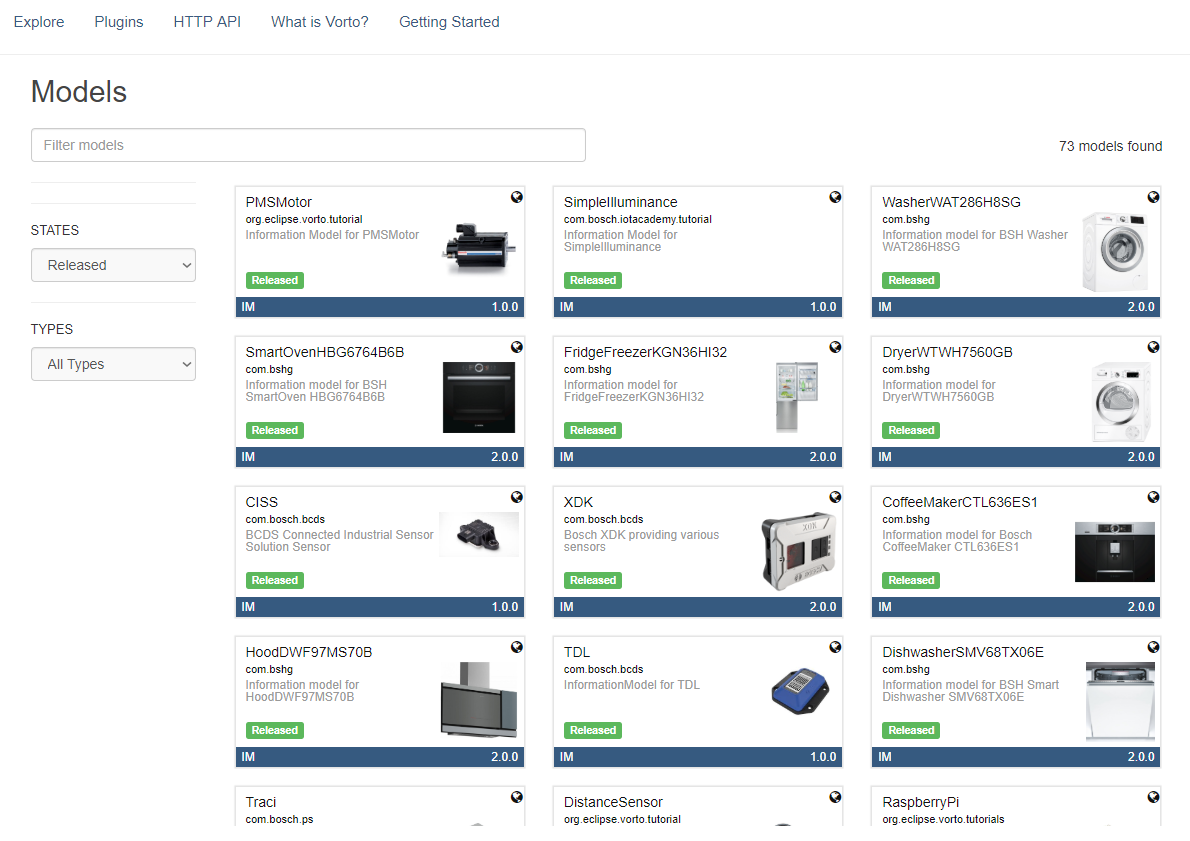
\includegraphics[width=1.3\textwidth]{img/EclipseVorto.png}
    \caption[Eclipse Vorto's device catalogue]{Screenshot of Eclipse Vorto's device catalogue. Every device has a self-explaining interface semantic. The catalogue is community based, i.e. everyone can add his or her device~\cite{Eclipse2019Vorto2019}.}
    \label{fig:vorto}
\end{figure}
\end{landscape}

Choosing an applicable ODM for a specific task can then be handled by the community through a rating system. If the user base is big enough, it will be possible to evaluate best practices for camera/ODM/machine/part type combinations.

Moreover, ODS can provide (hyperlinks to) tutorials and offer workshops alongside the ODS to better scale their know-how. The ODM source code does not have to be revealed with the advantage of a lower incentive to add content to the catalogue.

The challenge for this catalogue is to reach a critical mass (i.e., active users) to prosper.

\begin{figure}[ht]
    \centering
    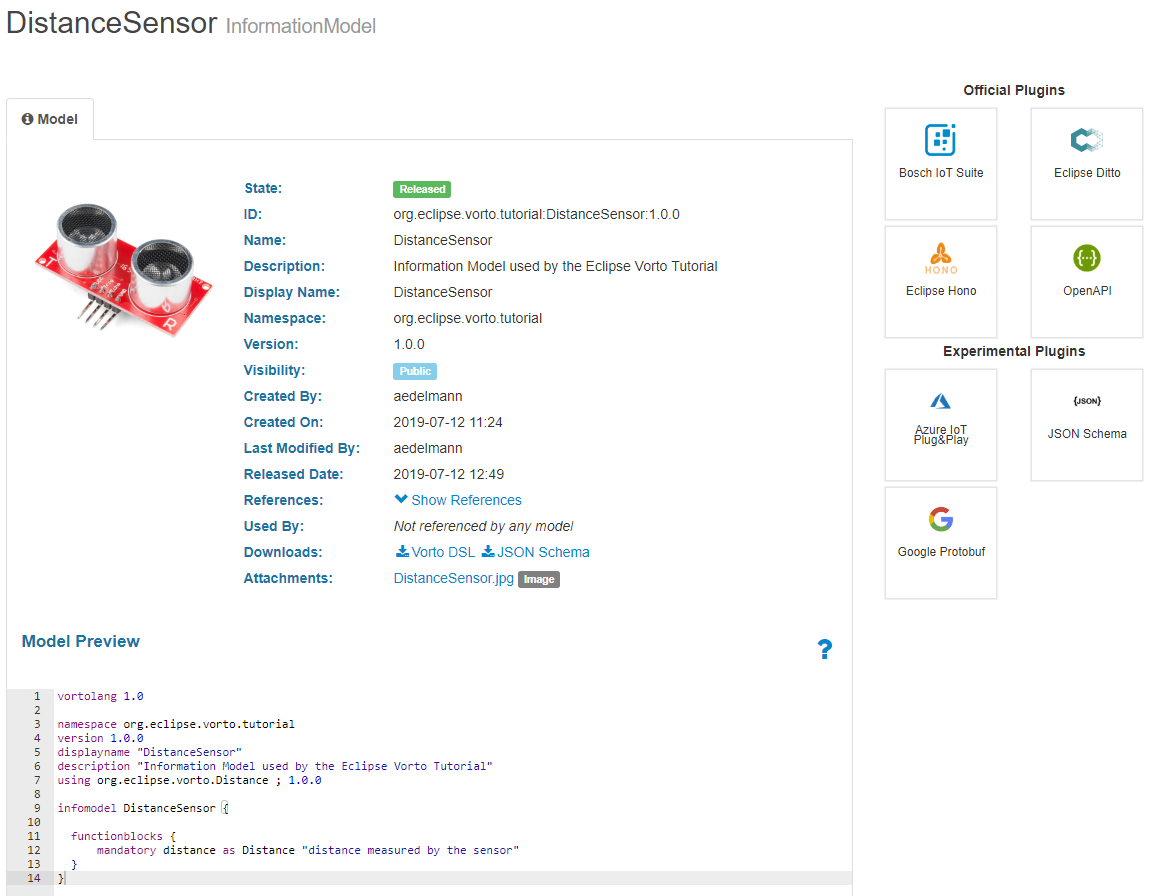
\includegraphics[width=\textwidth]{img/ScreenshotVortoDistanceSensor.png}
    \caption[Distance sensor in Eclipse Vorto's device catalogue]{Screenshot of a detail view of a distance sensor in Eclipse Vorto's device catalogue. Every device has a self-explaining interface semantic. Data types can be shared between devices~\cite{Eclipse2019Vorto2019}. Plugins for mapping to other interface definition languages such as Google Protobuf are available.}
    \label{fig:vorto2}
\end{figure}

\subsection{Handling Object Detection Services with Varying Interfaces}
RG uses gRPC for service communication. There is the possibility to offer a REST gateway~\cite{gRPC-Gateway-Documentation2017Grpc-gateway.2018} as well. This covers a broad range of (web-) services. Still, the framework highly depends on the ODS provider and his ODM configurability to interact with RG. Some ODS providers do not offer a gRPC interface. In this case, the REST gateway would also not find a remedy since it only maps REST to gRPC, not vice versa. Hence, for now RG mainly has to work with open-source ODM. 

Also, the services are dockerized. This is a convenient way of deployment for ODS that the RG user owns. RG does not yet however give possibility to utilize cloud-based pay-per-use ODS like Google cloud vision offers~\cite{Google-Cloud-Documentation2019Google2019-04-26}. This partly due to the interface semantic abstraction, but also on the protocol. A RG REST client would facilitate RG to work with most cloud-based services, not only the ones that support gRPC like GCV~\cite{Google-Cloud-Documentation2019Google2019-04-26}.

In the delimitation section of chapter~\ref{cha:chapter1} it was stated that this thesis will not cover real-time aspects. Nonetheless, it should not be disregarded in practice. Assuming TSN becomes a predominant technology in the next years, numerous aspects need to be considered. First, new hardware has to be purchased. That can be machines that are TSN-ready, network switches or network adapters. Moreover, the interface protocols need to be exchanged. As gRPC is a protocol designed for information technology, it focuses on being excessively fast - but not right on time. Lastly, the underlying ODsM need to be designed and tested against real-time requirements. To sum up, in the current state the framework can only be used for non time critical processes.

\subsection{Handling Object Detection Services with Varying Detection Methods}
RG's approach of coping with varying ODMs is abstraction. It is shown that modern complex ODMs basically comprise two phases - preparation (Train) and detection (Test). For RG to prosper, one party has to grasp every new ODM to adhere it to the two abstracted methods. That can only happen if the two methods are accepted as generic semantic interfaces. This calls for a standardization organization like the OPC foundation. RG can act as the spark of this fruitful thought. Taken into account how much cost and lock in effects arouse during the fieldbus war~\cite{Felser2002TheBattles}, it is particularly important to get together at an early stage.

RG further relies on strong decoupling of hardware and software. The ODMs can be configured with a file for calibration and OD optimization. When it is implemented, the ODM should be as concise as possible. 

The granularity of the services is another important domain that needs to be considered. Trading off between performance and reusability is the challenge here. Currently, RG delivers high performance due to coarse granularity~\cite{Rudorfer:2018:CSG:3284557.3284713}. Due to the strict pose output of the Test method, it is not possible to combine multiple ODMs for a greater task externally. However, the fine-granular services (e.g., edge detection) can be hidden behind the external method. As Docker offers a layered file system, new components can be added simply. This also implies that ODM providers to need do not need to expose their know how and can remain a propietary license.
